\section{App}

\subsection{Sichten}

\subsubsection{Visualisierung}
\label{sec:appSichtAnzeige}

\begin{wrapfigure}[16]{r}{0.5\textwidth}
  \begin{center}
	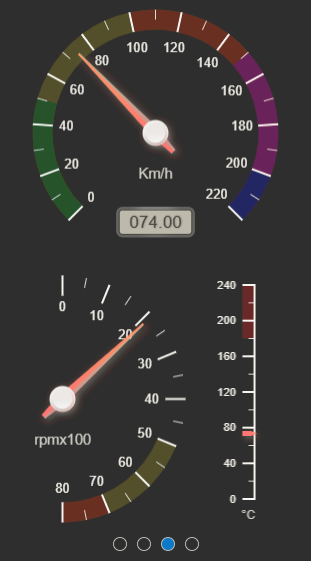
\includegraphics[width=0.3\textwidth]{./img/App_Speedo}
	\caption{Ansicht \enquote{Speedo}}
	\label{fig:App_Speedo}
  \end{center}
\end{wrapfigure}

In der Smartphone-App stehen mehrere Sichten für die Anzeige der Live Daten zur Verfügung. Diese können über eine Callback-Funktion auf schon vorbereite Daten vom Dongle und Smartphone zugreifen. Dadurch müssen sich diese nur noch um die bloße Darstellung der Daten kümmern. Jede Sicht fügt sich dabei selbst der Liste der Views hinzu und wird dadurch in der App angezeigt. So ist es ein Leichtes, sobald neue Daten vom Dongle zur Verfügung stehen sollten, fast unbegrenzt weitere Ansichten hinzuzufügen.
\\
Zurzeit stehen drei Sichten zur Auswahl. Eine einfache Liste mit allen vom Dongle und Smartphone verfügbaren Werten. Darunter die Geschwindigkeit, gemessen vom Dongle sowohl als auch vom Handy, Drehzahl, Kühlwassertemperatur und die GPS Daten des Dongles und Smartphones.
\\
Des weiteren eine Tachoansicht (siehe Abbildung \ref{fig:App_Speedo}), welche die momentan gefahrene Geschwindigkeit, Drehzahl und die Kühlwassertemperatur anzeigt.
\\ 
Die letzte zurzeit implementierte Sicht ist ein Vergleich der gemessenen Geschwindigkeit von der OBD-Schnittstelle und der ermittelten Geschwindigkeit vom GPS-Sensor. Diese sind jeweils als Tacho visualisiert.

\subsubsection{Konfiguration}
\label{sec:appSichtKonfiguration}

Die \enquote{Konfiguration View} (siehe Abbildung \ref{fig:APP_Configuration}a) ist eine spezielle Sicht, in der unter anderem die Verbindung zum Dongle hergestellt werden kann. Dazu steht ein Dialog (siehe Abbildung \ref{fig:APP_Configuration}b) zum Suchen aller in der Umgebung befindlichen Bluetooth-Geräte zur Verfügung. Beim Anklicken wird versucht eine Verbindung zu diesem Device aufzubauen. Durch Klicken auf den Button \enquote{Test} kann geprüft werden, ob zurzeit eine Verbindung zu diesem besteht. Das gleiche Prinzip ist auch für die Verbindung zum Backend vorhanden. Hier öffnet sich beim Button \enquote{Connect} eine Liste der Verbindungsparameter, die dazu benötigt werden. Außerdem sind in dieser Sicht noch die App-Einstellungen (z.B Km/H oder Mp/H) änderbar und die Logging-Liste auslesbar.

\begin{figure}[H]
	\centering 
	\subfigure[Übersicht]{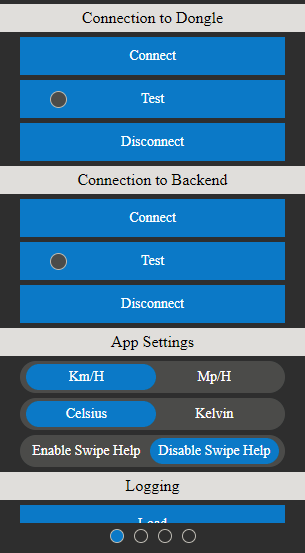
\includegraphics[width=0.3\textwidth]{./img/APP_Configuration}}
    \label{fig:APP_Configuration_View}
    \hspace{1cm}
	\subfigure[Dialog \enquote{Dongle - Connect}]{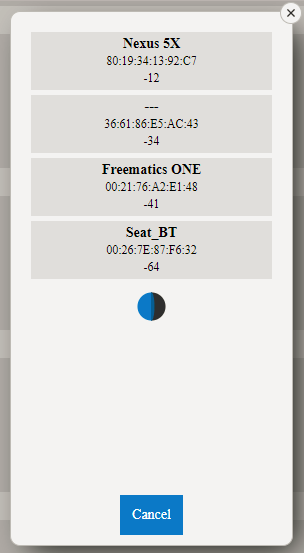
\includegraphics[width=0.3\textwidth]{./img/App_Bluetooth_Search}}
	\label{fig:App_Bluetooth_Search}
	\caption{Ansicht \enquote{Konfiguration}}
	\label{fig:APP_Configuration}
\end{figure}

\subsection{Bluetooth}
\label{sec:appBluetooth}

Die Kommunikation mit dem Dongle erfolgt über Bluetooth Low Energy. Dafür wurde in der App das Cordova-Plugin \enquote{ble-central} verwendet. Das Plugin dient als einfacher \enquote{Wrapper} zu den nativen Funktionen. Außerdem mussten spezielle BLE-Konventionen eingehaltet werden. So können Daten nur durch das Abonnieren vom Sender angebotener \enquote{Characteristic}s (32 Bit ID) von \enquote{Service}s (32 Bit ID) empfangen und gesendet werden. Welche \enquote{Service}s und \enquote{Characteristic}s angeboten werden, müssen vorher angefragt  werden. Hierbei gibt es zum einen Standard-Services (z.B. Device Information - 0x180A) und zum anderen Custom-Services zum Übertragen von speziellen Daten. Das Bluetooth Modul vom Dongle ist nicht veränderbar und sendet alle Daten, die über die serielle Konsole gesendet werden über den Service 0xFFE0 und der Characteristic 0xFFE1. Dadurch kann das für BLE empfohlene Schema, das Trennen der Daten durch andere Characteristic-ID, nicht angewandt werden. Somit muss für die unterschiedlichen Anforderungen weitere Merkmale zur Unterscheidung der Daten eingebaut werden.\cite{BluetoothLowEnergy}
\\
Wie auch bei normalen TCP-Netzwerkkommunikation können bei Bluetooth die Daten in Pakete aufgeteilt werden. In diesem Fall müssen die Daten beim Empfangen wieder zusammengesetzt werden. Falls in einem Callback festgestellt wird, dass ein Datensatz nicht vollständig angekommen ist, wird dieser Teil vom Puffer des aktuellen Callback's entfernt und dem Zukünftigen am Anfang hinzugefügt.

\subsection{GPS}
\label{sec:appGPS}

Um einen Vergleich der Genauigkeit des GPS-Sensors im Dongle zu erhalten, wird dieser mit dem GPS-Sensor des Smartphones verglichen. Dazu wird entweder die letzte gespeicherte Position des Betriebssystems genutzt, falls diese nicht länger als 10 Sekunden alt ist, oder eine neue Position angefordert.

\subsection{Zugriff auf Identity Server}

Um mit den Backend kommunizieren zu können, muss zuerst die Authentifizierung über den Identity Server stattfinden. Dieser bietet dafür mehrere Möglichkeiten (z.B. Authorization Code, Client Credentials). In der App wird die Authentifizierungsmethode \enquote{Password Grand} verwendet. Dabei wird ein JSON-Objekt (siehe nachfolgenden Code) über einen HTTP-Request, mit Hilfe von AJAX, an den Server gesendet. Das Objekt enthält den Namen und das Passwort des Benutzers, sowie eine Client ID, die extra für die APP ausgestellt wurde, und ein dazu passendes Geheimnis. Der Authentifizierungsserver liefert nun ein Token zurück, mit dem nun mit dem Backend für eine gewisse Zeit kommuniziert werden kann. Dieses wird dem Backend bei jedem Request über dem HTTP Header mitgesendet. \cite{RFC6749}\cite{RFC6750}

\noindent
\begin{minipage}{\linewidth} 
\begin{lstlisting}
{
	username: Store.get(username), 
	password: Store.get(password),
	scope: "openid",
	grant_type: "password",
	client_id: Settings.Backend.clientId,
	client_secret: Settings.Backend.secret
}
\end{lstlisting} 
\end{minipage}

\subsection{Konfiguration}
\label{sec:appKonfiguration}

Es gibt Grundlegend drei Arten von Konfigurationswerten. Zum einen statische, Standard- und Initial- Werte (z.B Timeouts, Client ID / Secret, Standard Ansicht), die fest im Code integriert sind. Diese sind zur besseren Wartbarkeit in der Datei \enquote{Settings} als JSON-Objekt gesammelt. Veränderbare Einstellungen können entweder im \enquote{Local Store} oder im \enquote{Session Store} als Key-Value-Paar angelegt werden. Dabei sind sie entweder flüchtig (z.B. für den Token), damit zeitlich begrenzt gelöscht, oder fest (z.B. für die Sprache) gespeichert.

\subsection{Mehrsprachigkeit}
\label{sec:appMehrsprachigkeit}

Um die geforderte Mehrsprachigkeit zu gewährleisten, sind alle verwendeten Texte in einer JSON-Datei zusammengefasst. In dieser sind die Texte als Key-Value-Paar abgespeichert (z.B. load: „load“); falls der beinhaltende Text eine Übersetzung benötigt, kann das Key-Value-Paar optional in die jeweiligen Sprachen aufgeteilt werden (z.B.
load: \{ en: „load“, de: „laden“ \}). Die \enquote{String}-Klasse ermittelt dann mit Hilfe der eingestellten Sprache den zu verwendenden Text. Falls der Text in der aktuellen Sprache nicht verfügbar ist, wird die Standardsprache (Englisch) zurückgegeben.

\pagebreak

\subsection{Weitere Anzeigeelemente}
\label{sec:appAnzeigeelemente}

\begin{wrapfigure}{R}{0.45\textwidth}
  \begin{center}
	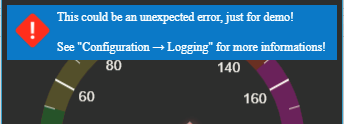
\includegraphics[width=0.4\textwidth]{./img/App_ErrorPanel}
	\caption{Error Panel}
	\label{fig:App_ErrorPanel}
	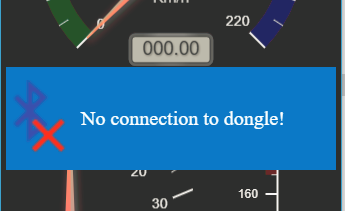
\includegraphics[width=0.4\textwidth]{./img/App_NoConnectionPanel}
	\caption{No Connection Panel}
	\label{fig:App_NoConnectionPanel}
    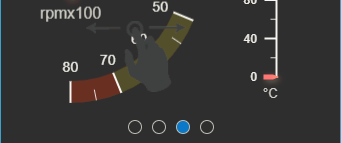
\includegraphics[width=0.4\textwidth]{./img/App_SwipeHelp}
    \caption{Swipe Help}
    \label{fig:App_SwipeHelp}
    
\includegraphics[width=0.4\textwidth]{./img/App_ViewCircles}
    \caption{View Circles}
    \label{fig:App_ViewCircles}
    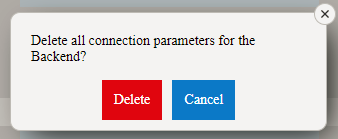
\includegraphics[width=0.4\textwidth]{./img/App_Dialog}
    \caption{Dialog}
    \label{fig:App_Dialog}
  \end{center}
\end{wrapfigure}

Für das Anzeigen von speziellen Informationen gibt es mehrere Elemente. Zur Mitteilung von unerwarteten Fehlern gibt es einen Fehler Dialog (siehe Abbildung \ref{fig:App_ErrorPanel}). Dieses zeigt am oberen Rand des Bildschirmes eine Kurzinformation zum Fehler und die Information, dass sie im Logging-Bereich der Konfigurationsansicht komplett eingesehen werden kann an.
\\
Falls keine Bluetooth Verbindung zum Dongle besteht oder diese abgebrochen oder gestört ist, wird im mittleren Teil des Displays ein Panel (siehe Abbildung \ref{fig:App_NoConnectionPanel}) angezeigt, das dieses Ereignis visualisiert.
\\
Für die erste Benutzung der App wird beim Starten der App eine bewegende Anzeige (siehe Abbildung \ref{fig:App_SwipeHelp}) eingeblendet, die den Anwender signalisieren soll, dass durch nach Links und Rechts wischen weitere Ansichten und Optionen zur Verfügung stehen. Diese Funktion kann, falls sie als Störend empfunden wird, in der Konfigurationssicht deaktiviert werden. 
\\
Um den Benutzer über die gerade angezeigt Sicht zu informieren, sind am unteren Ende der App Kreise (siehe Abbildung \ref{fig:App_ViewCircles}) für jede View symbolisiert. Der Kreis für die zurzeit sichtbare Ansicht ist dabei ausgefüllt.
\\
Für manche Funktionen bieten sich Dialoge am besten an. Hier gibt es zum einen kleine Dialoge wie in Abbildung \ref{fig:App_ViewCircles} zu sehen und zum anderen Fullscreen-Dialoge, für zum Beispiel das Suchen der aktuellen Bluetooth Geräte im Umkreis (siehe Kapitel \ref{sec:appSichtKonfiguration}).


 
 
 
 
